\documentclass{standalone}
\usepackage{tikz}
\usetikzlibrary{patterns, positioning}


\begin{document}
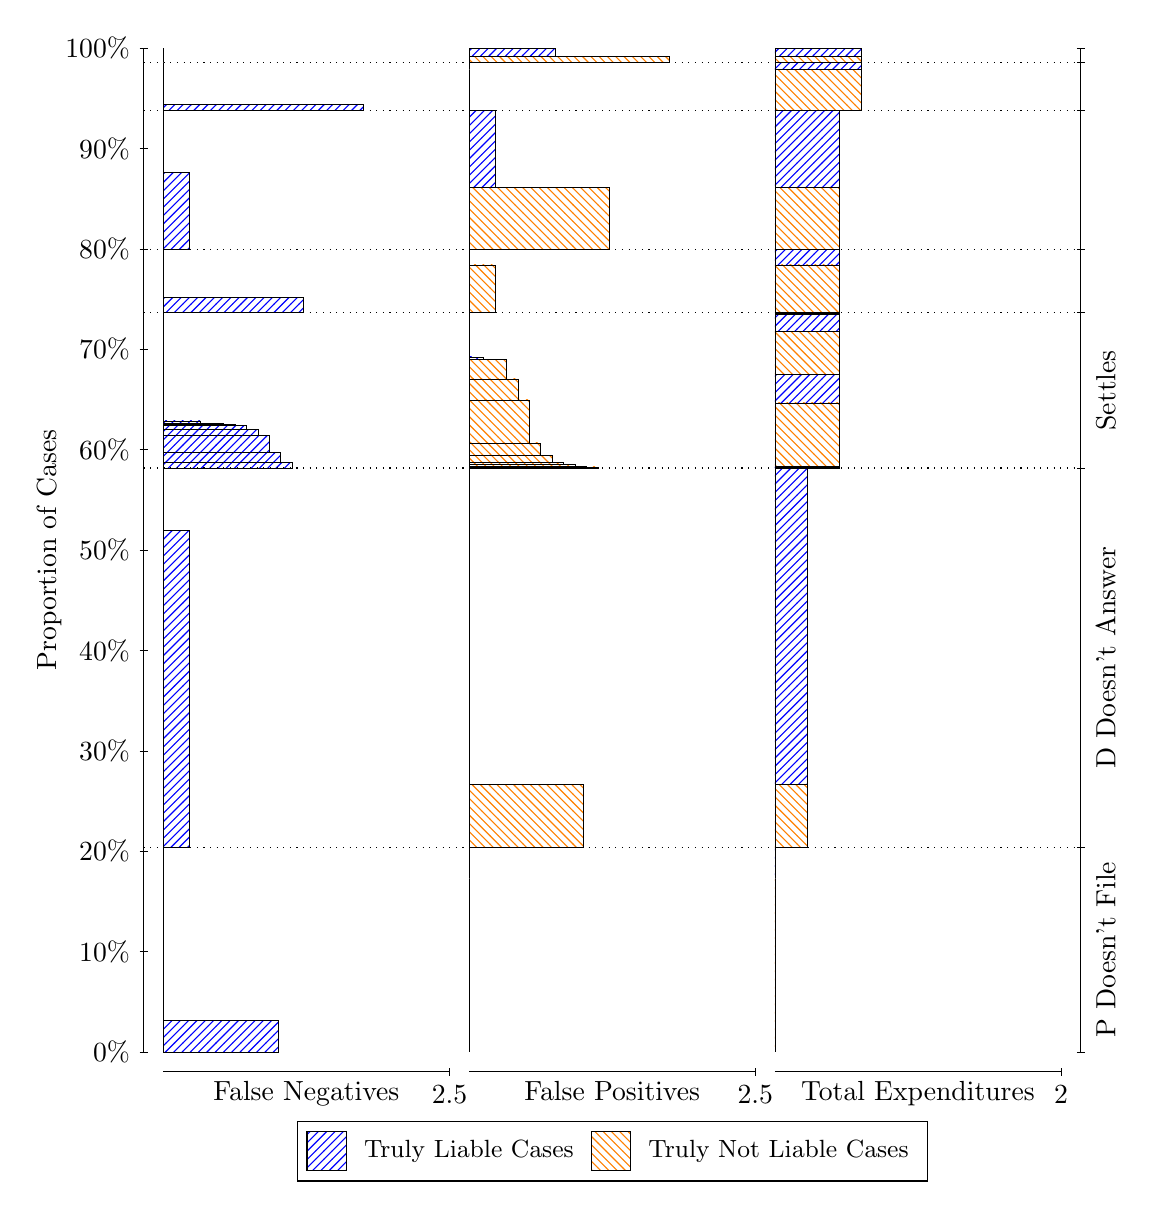
\begin{tikzpicture}
\draw[black, very thin] (1.5,1.75) -- (1.5,14.5);
\node[rotate=90, text=black, anchor=center] at (0.3, 8.125) {Proportion of Cases};
\draw[black, very thin] (1.45,1.75) -- (1.55,1.75);
\node[text=black, anchor=east] at (1.45, 1.75) {0\%};
\draw[black, very thin] (1.45,3.025) -- (1.55,3.025);
\node[text=black, anchor=east] at (1.45, 3.025) {10\%};
\draw[black, very thin] (1.45,4.3) -- (1.55,4.3);
\node[text=black, anchor=east] at (1.45, 4.3) {20\%};
\draw[black, very thin] (1.45,5.575) -- (1.55,5.575);
\node[text=black, anchor=east] at (1.45, 5.575) {30\%};
\draw[black, very thin] (1.45,6.85) -- (1.55,6.85);
\node[text=black, anchor=east] at (1.45, 6.85) {40\%};
\draw[black, very thin] (1.45,8.125) -- (1.55,8.125);
\node[text=black, anchor=east] at (1.45, 8.125) {50\%};
\draw[black, very thin] (1.45,9.4) -- (1.55,9.4);
\node[text=black, anchor=east] at (1.45, 9.4) {60\%};
\draw[black, very thin] (1.45,10.675) -- (1.55,10.675);
\node[text=black, anchor=east] at (1.45, 10.675) {70\%};
\draw[black, very thin] (1.45,11.95) -- (1.55,11.95);
\node[text=black, anchor=east] at (1.45, 11.95) {80\%};
\draw[black, very thin] (1.45,13.225) -- (1.55,13.225);
\node[text=black, anchor=east] at (1.45, 13.225) {90\%};
\draw[black, very thin] (1.45,14.5) -- (1.55,14.5);
\node[text=black, anchor=east] at (1.45, 14.5) {100\%};

\draw[black, very thin] (13.4,1.75) -- (13.4,14.5);
\draw[black, very thin] (13.35,1.75) -- (13.45,1.75);
\node[anchor=west] at (13.35, 1.75) {};
\draw[black, very thin] (13.35,4.3498) -- (13.45,4.3498);
\node[anchor=west] at (13.35, 4.3498) {};
\draw[black, very thin] (13.35,9.1668) -- (13.45,9.1668);
\node[anchor=west] at (13.35, 9.1668) {};
\draw[black, very thin] (13.35,11.14) -- (13.45,11.14);
\node[anchor=west] at (13.35, 11.14) {};
\draw[black, very thin] (13.35,11.941) -- (13.45,11.941);
\node[anchor=west] at (13.35, 11.941) {};
\draw[black, very thin] (13.35,13.704) -- (13.45,13.704);
\node[anchor=west] at (13.35, 13.704) {};
\draw[black, very thin] (13.35,14.315) -- (13.45,14.315);
\node[anchor=west] at (13.35, 14.315) {};
\draw[black, very thin] (13.35,14.5) -- (13.45,14.5);
\node[anchor=west] at (13.35, 14.5) {};

\draw[black, very thin, pattern color=blue, pattern=north east lines] (1.75,1.75) rectangle (3.2033,2.1496);
\draw[black, very thin, pattern color=orange, pattern=north west lines] (1.75,2.1496) rectangle (1.75,4.3498);
\draw[black, very thin, pattern color=blue, pattern=north east lines] (1.75,4.3498) rectangle (2.077,8.3693);
\draw[black, very thin, pattern color=orange, pattern=north west lines] (1.75,8.3693) rectangle (1.75,9.1668);
\draw[black, very thin, pattern color=blue, pattern=north east lines] (1.75,9.1668) rectangle (3.385,9.2351);
\draw[black, very thin, pattern color=blue, pattern=north east lines] (1.75,9.2351) rectangle (3.2397,9.3617);
\draw[black, very thin, pattern color=blue, pattern=north east lines] (1.75,9.3617) rectangle (3.0943,9.5819);
\draw[black, very thin, pattern color=blue, pattern=north east lines] (1.75,9.5819) rectangle (2.949,9.6549);
\draw[black, very thin, pattern color=blue, pattern=north east lines] (1.75,9.6549) rectangle (2.8037,9.7062);
\draw[black, very thin, pattern color=blue, pattern=north east lines] (1.75,9.7062) rectangle (2.6583,9.7184);
\draw[black, very thin, pattern color=blue, pattern=north east lines] (1.75,9.7184) rectangle (2.513,9.73);
\draw[black, very thin, pattern color=blue, pattern=north east lines] (1.75,9.73) rectangle (2.3677,9.7371);
\draw[black, very thin, pattern color=blue, pattern=north east lines] (1.75,9.7371) rectangle (2.2223,9.7639);
\draw[black, very thin, pattern color=orange, pattern=north west lines] (1.75,9.7639) rectangle (1.75,11.14);
\draw[black, very thin, pattern color=blue, pattern=north east lines] (1.75,11.14) rectangle (3.5303,11.335);
\draw[black, very thin, pattern color=orange, pattern=north west lines] (1.75,11.335) rectangle (1.75,11.941);
\draw[black, very thin, pattern color=blue, pattern=north east lines] (1.75,11.941) rectangle (2.077,12.918);
\draw[black, very thin, pattern color=orange, pattern=north west lines] (1.75,12.918) rectangle (1.75,13.704);
\draw[black, very thin, pattern color=blue, pattern=north east lines] (1.75,13.704) rectangle (4.2933,13.789);
\draw[black, very thin, pattern color=orange, pattern=north west lines] (1.75,13.789) rectangle (1.75,14.315);
\draw[black, very thin, pattern color=orange, pattern=north west lines] (1.75,14.315) rectangle (1.75,14.398);
\draw[black, very thin, pattern color=blue, pattern=north east lines] (1.75,14.398) rectangle (1.75,14.5);
\draw[black, very thin, pattern color=orange, pattern=north west lines] (5.6333,1.75) rectangle (5.6333,3.9502);
\draw[black, very thin, pattern color=blue, pattern=north east lines] (5.6333,3.9502) rectangle (5.6333,4.3498);
\draw[black, very thin, pattern color=orange, pattern=north west lines] (5.6333,4.3498) rectangle (7.0867,5.1473);
\draw[black, very thin, pattern color=blue, pattern=north east lines] (5.6333,5.1473) rectangle (5.6333,9.1668);
\draw[black, very thin, pattern color=orange, pattern=north west lines] (5.6333,9.1668) rectangle (7.2683,9.1818);
\draw[black, very thin, pattern color=orange, pattern=north west lines] (5.6333,9.1818) rectangle (7.123,9.1908);
\draw[black, very thin, pattern color=orange, pattern=north west lines] (5.6333,9.1908) rectangle (6.9777,9.208);
\draw[black, very thin, pattern color=orange, pattern=north west lines] (5.6333,9.208) rectangle (6.8323,9.2366);
\draw[black, very thin, pattern color=orange, pattern=north west lines] (5.6333,9.2366) rectangle (6.687,9.328);
\draw[black, very thin, pattern color=orange, pattern=north west lines] (5.6333,9.328) rectangle (6.5417,9.4844);
\draw[black, very thin, pattern color=orange, pattern=north west lines] (5.6333,9.4844) rectangle (6.3963,10.032);
\draw[black, very thin, pattern color=orange, pattern=north west lines] (5.6333,10.032) rectangle (6.251,10.298);
\draw[black, very thin, pattern color=orange, pattern=north west lines] (5.6333,10.298) rectangle (6.1057,10.543);
\draw[black, very thin, pattern color=blue, pattern=north east lines] (5.6333,10.543) rectangle (5.815,10.569);
\draw[black, very thin, pattern color=blue, pattern=north east lines] (5.6333,10.569) rectangle (5.6697,10.577);
\draw[black, very thin, pattern color=blue, pattern=north east lines] (5.6333,10.577) rectangle (5.6333,11.14);
\draw[black, very thin, pattern color=orange, pattern=north west lines] (5.6333,11.14) rectangle (5.9603,11.746);
\draw[black, very thin, pattern color=blue, pattern=north east lines] (5.6333,11.746) rectangle (5.6333,11.941);
\draw[black, very thin, pattern color=orange, pattern=north west lines] (5.6333,11.941) rectangle (7.4137,12.727);
\draw[black, very thin, pattern color=blue, pattern=north east lines] (5.6333,12.727) rectangle (5.9603,13.704);
\draw[black, very thin, pattern color=orange, pattern=north west lines] (5.6333,13.704) rectangle (5.6333,14.23);
\draw[black, very thin, pattern color=blue, pattern=north east lines] (5.6333,14.23) rectangle (5.6333,14.315);
\draw[black, very thin, pattern color=orange, pattern=north west lines] (5.6333,14.315) rectangle (8.1767,14.398);
\draw[black, very thin, pattern color=blue, pattern=north east lines] (5.6333,14.398) rectangle (6.7233,14.5);
\draw[black, very thin, pattern color=orange, pattern=north west lines] (9.5167,1.75) rectangle (9.5167,3.9502);
\draw[black, very thin, pattern color=blue, pattern=north east lines] (9.5167,3.9502) rectangle (9.5167,4.3498);
\draw[black, very thin, pattern color=orange, pattern=north west lines] (9.5167,4.3498) rectangle (9.9254,5.1473);
\draw[black, very thin, pattern color=blue, pattern=north east lines] (9.5167,5.1473) rectangle (9.9254,9.1668);
\draw[black, very thin, pattern color=orange, pattern=north west lines] (9.5167,9.1668) rectangle (10.334,9.1785);
\draw[black, very thin, pattern color=blue, pattern=north east lines] (9.5167,9.1785) rectangle (10.334,9.1843);
\draw[black, very thin, pattern color=orange, pattern=north west lines] (9.5167,9.1843) rectangle (10.334,9.9922);
\draw[black, very thin, pattern color=blue, pattern=north east lines] (9.5167,9.9922) rectangle (10.334,10.356);
\draw[black, very thin, pattern color=orange, pattern=north west lines] (9.5167,10.356) rectangle (10.334,10.903);
\draw[black, very thin, pattern color=blue, pattern=north east lines] (9.5167,10.903) rectangle (10.334,11.124);
\draw[black, very thin, pattern color=orange, pattern=north west lines] (9.5167,11.124) rectangle (10.334,11.133);
\draw[black, very thin, pattern color=blue, pattern=north east lines] (9.5167,11.133) rectangle (10.334,11.14);
\draw[black, very thin, pattern color=orange, pattern=north west lines] (9.5167,11.14) rectangle (10.334,11.746);
\draw[black, very thin, pattern color=blue, pattern=north east lines] (9.5167,11.746) rectangle (10.334,11.941);
\draw[black, very thin, pattern color=orange, pattern=north west lines] (9.5167,11.941) rectangle (10.334,12.727);
\draw[black, very thin, pattern color=blue, pattern=north east lines] (9.5167,12.727) rectangle (10.334,13.704);
\draw[black, very thin, pattern color=orange, pattern=north west lines] (9.5167,13.704) rectangle (10.607,14.23);
\draw[black, very thin, pattern color=blue, pattern=north east lines] (9.5167,14.23) rectangle (10.607,14.315);
\draw[black, very thin, pattern color=orange, pattern=north west lines] (9.5167,14.315) rectangle (10.607,14.398);
\draw[black, very thin, pattern color=blue, pattern=north east lines] (9.5167,14.398) rectangle (10.607,14.5);
\draw[black, dotted] (1.5,4.3498) -- (13.4,4.3498);
\draw[black, dotted] (1.5,9.1668) -- (13.4,9.1668);
\draw[black, dotted] (1.5,11.14) -- (13.4,11.14);
\draw[black, dotted] (1.5,11.941) -- (13.4,11.941);
\draw[black, dotted] (1.5,13.704) -- (13.4,13.704);
\draw[black, dotted] (1.5,14.315) -- (13.4,14.315);
\draw[black, very thin] (1.75,1.5) -- (5.3833,1.5);
\node[text=black, anchor=north] at (3.5667, 1.5) {False Negatives};
\draw[black, very thin] (5.3833,1.45) -- (5.3833,1.55);
\node[text=black, anchor=north] at (5.3833, 1.45) {2.5};

\draw[black, very thin] (5.6333,1.5) -- (9.2667,1.5);
\node[text=black, anchor=north] at (7.45, 1.5) {False Positives};
\draw[black, very thin] (9.2667,1.45) -- (9.2667,1.55);
\node[text=black, anchor=north] at (9.2667, 1.45) {2.5};

\draw[black, very thin] (9.5167,1.5) -- (13.15,1.5);
\node[text=black, anchor=north] at (11.333, 1.5) {Total Expenditures};
\draw[black, very thin] (13.15,1.45) -- (13.15,1.55);
\node[text=black, anchor=north] at (13.15, 1.45) {2};

\node[text=black, centered, rotate=90] at (13.72, 3.0499) {P Doesn't File};
\node[text=black, centered, rotate=90] at (13.72, 6.7583) {D Doesn't Answer};
\node[text=black, centered, rotate=90] at (13.72, 10.153) {Settles};





\draw (7.449999999999999,1.5) node[draw=none] (baseCoordinate) {};
\begin{scope}[align=center]
        \matrix[scale=0.5, draw=black, below=0.5cm of baseCoordinate, nodes={draw}, column sep=0.1cm]{
            \node[rectangle, draw, minimum width=0.5cm, minimum height=0.5cm, pattern color=blue, pattern=north east lines] {}; &
            \node[draw=none, font=\small, text=black] (B) {Truly Liable Cases}; &
            \node[rectangle, draw, minimum width=0.5cm, minimum height=0.5cm, pattern color=orange, pattern=north west lines] {}; &
            \node[draw=none, font=\small, text=black] (B) {Truly Not Liable Cases}; \\
            };
\end{scope}

\end{tikzpicture}
\end{document}